\documentclass[../../main/main.tex]{subfiles}
\graphicspath{{./figures/}}

\setlength{\mtcindent}{-10pt}
\mtcsetoffset{minitoc}{-10pt}

\dominitoc
\faketableofcontents

\makeatletter
\renewcommand{\@chapapp}{Ondes -- chapitre}
\makeatother

% \toggletrue{student}
\HideSolutionstrue
\toggletrue{corrige}
% \renewcommand{\mycol}{black}
\renewcommand{\mycol}{gray}

\begin{document}
\setcounter{chapter}{0}

\chapter{Ondes progressives}

\vfill

\begin{prgm}
	\begin{tcb}*(ror)"know"{Savoirs}
		\begin{itemize}[label=$\diamond$, leftmargin=10pt]
			\item Identifier les grandeurs physiques correspondant à
			      des signaux acoustiques, électriques, électromagnétiques.
			\item Propagation d'un signal dans un milieu illimité, non dispersif et
			      transparent.
			\item Onde progressive dans le cas d'une propagation unidimensionnelle non
			      dispersive.
			\item Modèle de l'onde progressive sinusoïdale unidimensionnelle. Vitesse
			      de phase, déphasage, double périodicité spatiale et temporelle.
			\item Définir un milieu dispersif. Citer des exemples de situations de
			      propagation dispersive et non dispersive.
			\item Citer quelques ordres de grandeur de fréquences dans les domaines
			      acoustique, mécanique et électromagnétique.
		\end{itemize}
	\end{tcb}
	\begin{tcb}*(ror)"how"{Savoir-faire}
		\begin{itemize}[label=$\diamond$, leftmargin=10pt]
			\item Écrire les signaux sous la forme $f(x-ct)$ ou $g(x+ct)$, et
			      sous la forme $f(t-x/c)$ ou $g(t+x/c)$.
			\item Prévoir, dans le cas d'une onde progressive, l'évolution temporelle
			      à position fixée et l'évolution spatiale à différents instants.
			\item Établir la relation entre la fréquence, la longueur d'onde et la
			      vitesse de phase.
			\item Relier le déphasage entre les signaux perçus en deux points
			      distincts au retard dû à la propagation.
		\end{itemize}
	\end{tcb}
\end{prgm}

\vfill

\newpage

\vspace*{\fill}
% \vfill
\minitoc
% \vfill
\vspace*{\fill}

\newpage

%Tension et vitesse en fonction du milieu~: \url{https://phet.colorado.edu/sims/html/wave-on-a-string/latest/wave-on-a-string_fr.html}

\section{Introduction}
\subsection{Signal}
\begin{tcb}(defi)<lft>'l'{\tiny Définition}
	On appelle \textbf{signal} une grandeur physique mesurable pouvant varier
	dans le temps et qui transporte une information.
\end{tcb}
\begin{tcb}(exem)<lft>'l'{Exemples}
	\begin{itemize}
		\item Signal \textbf{sonore}~: voix, instrument de musique~;
		\item Signal sismique~;
		\item Signal électrique…
	\end{itemize}
\end{tcb}
À noter que la notion de signal ou d'information \textbf{dépend de
	l'observation}. Les ondes radio servent bien sûr à écouter la radio, mais au
départ leur découverte était perturbée par le premier signal lumineux de
l'Univers, le fonds diffus cosmologique~: il baigne la totalité de l'Univers et
est fondamental dans la cosmologie, mais peut être parasite selon l'objectif.

\subsection{Perturbation}

\begin{tcb}(defi)<lft>'l'{\tiny Définition}
	Une \textbf{perturbation} est une modification locale et temporaire des
	propriétés d'un milieu.
\end{tcb}
\begin{tcb}(exem)<lft>'l'{Exemples}
	\begin{itemize}
		\item Jet d'un caillou dans un lac~;
		\item Séisme~;
		\item Déplacement de la membrane d'un haut-parleur…
	\end{itemize}
\end{tcb}
Une perturbation, quand elle est créée, se propage autour d'elle de proche en
proche~: chaque point impacté va subir des modifications temporaires similaires
à celle de la source. Après le passage de cette perturbation, chaque point
retrouve sa position initiale.

\subsection{Onde}
\begin{tcb}(defi){Définition}
	\psw{
		On appelle \textbf{onde} la propagation d'une perturbation, dans un milieu
		matériel ou dans le vide.
	}
\end{tcb}

Certaines ondes ont besoin d'un milieu matériel pour se propager~: ce sont les
ondes \textbf{mécaniques}. Les ondes sismiques, les ondes dans la corde ou les
ondes sonores en sont des exemples. Certaines ondes peuvent se propager dans le
vide, comme les ondes \textbf{électromagnétiques}. Les infrarouges, la lumière
visible ou les micro-ondes sont des exemples d'ondes électromagnétiques.

\begin{tcb}(exem)<lft>'l'{Exemples}
	\begin{itemize}
		\item Lorsqu'on secoue l'extrémité d'une corde tendue,
		      les positions des différents points sont modifiées. Une fois l'onde
		      passée, les points retrouvent leur position initiale.
		\item Le caillou dans le lac forme des \textbf{rides qui s'éloignent} du point
		      d'impact, mais il n'y a pas de mouvement d'ensemble du
		      fluide.
		\item La membrane du haut-parleur, lors de son déplacement elle provoque
		      une brève \textbf{compression-dilatation} de l'air qui la touche.
		      Cette propagation se déplace ensuite dans l'air~: ce sont les ondes
		      sonores. Elles peuvent aussi se déplacer dans les liquides et dans
		      les solides.
	\end{itemize}
\end{tcb}

\subsection{Perturbation et propagation}

La perturbation se propageant peut être soit parallèle, soit perpendiculaire à
la direction de propagation. On distingue donc~:

\begin{tcb}(defi){Définition}
	\begin{itemize}
		\bitem{Onde transversale}\footnote{\url{https://phyanim.sciences.univ-nantes.fr/Ondes/general/onde_transversale.php}}~:
		\psw{
			la perturbation est perpendiculaire à la direction de propagation~;
		}
		\bitem{Onde longitudunale}\footnote{\url{https://phyanim.sciences.univ-nantes.fr/Ondes/general/onde_longitudinale.php}}~:
		\psw{
			la perturbation est parallèle à la direction de propagation.
		}
	\end{itemize}
\end{tcb}

\begin{tcb}(exem)<lft>'l'{Exemples}
	\begin{minipage}{0.50\linewidth}
		\begin{itemize}
			\bitem{Longitudinales}~:
			\psw{
				\begin{itemize}
					\item Certaines ondes sismiques~;
					\item Contraction-élongation d'un ressort.
				\end{itemize}
			}
		\end{itemize}
	\end{minipage}
	\hfill
	\begin{minipage}{0.48\linewidth}
		\begin{itemize}
			\bitem{Transversales}~:
			\psw{
				\begin{itemize}
					\item Mouvement d'une corde secouée~;
					\item Vagues sur l'eau.
				\end{itemize}
			}
		\end{itemize}
	\end{minipage}
	\vspace{-15pt}
\end{tcb}

\section{Onde progressive à une dimension}
\subsection{Définition}
\begin{tcb}(defi){Définitions}
	\begin{itemize}
		\bitem{Progressive}~:
		\psw{
			sa propagation ne se fait que \textbf{dans un seul sens depuis sa source}.
			À un instant ultérieur, on retrouve la perturbation \textit{à l'identique
				plus loin}.
		}
		\bitem{À une dimension}~:
		\begin{itemize}
			\item
			      \psw{
				      une onde qui se propage dans un milieu matériel à une dimension~;
			      }
			\item
			      \psw{
				      ou une onde qui se propage dans un milieu matériel à deux ou trois
				      dimensions, avec une direction de propagation unique.
			      }
		\end{itemize}
	\end{itemize}
\end{tcb}

\begin{tcb}(exem)<lft>'l'{Exemples}
	\begin{itemize}
		\bitem{1D}~:
		\psw{
			onde le long d'une corde, compression le long d'un ressort~;
		}
		\bitem{2D}~:
		\psw{
			vagues sur l'eau~;
		}
		\bitem{3D}~:
		\psw{
			son, lumière.
		}
	\end{itemize}
	\vspace{-15pt}
\end{tcb}

\subsection{Représentation spatiale et célérité des ondes}

\begin{tcb}[sidebyside, lefthand ratio=.45](ror){Définition}
	\psw{
		Dans une représentation \textbf{spatiale}, on regarde à un \textbf{temps
			fixé} la perturbation dans \textbf{tout l'espace}~; on parle également de
		représentation \textbf{photographique}%
		\footnote{\url{https://phyanim.sciences.univ-nantes.fr/Ondes/general/retard.php}}.
	}
	\tcblower
	\begin{center}
		\sswitch{
			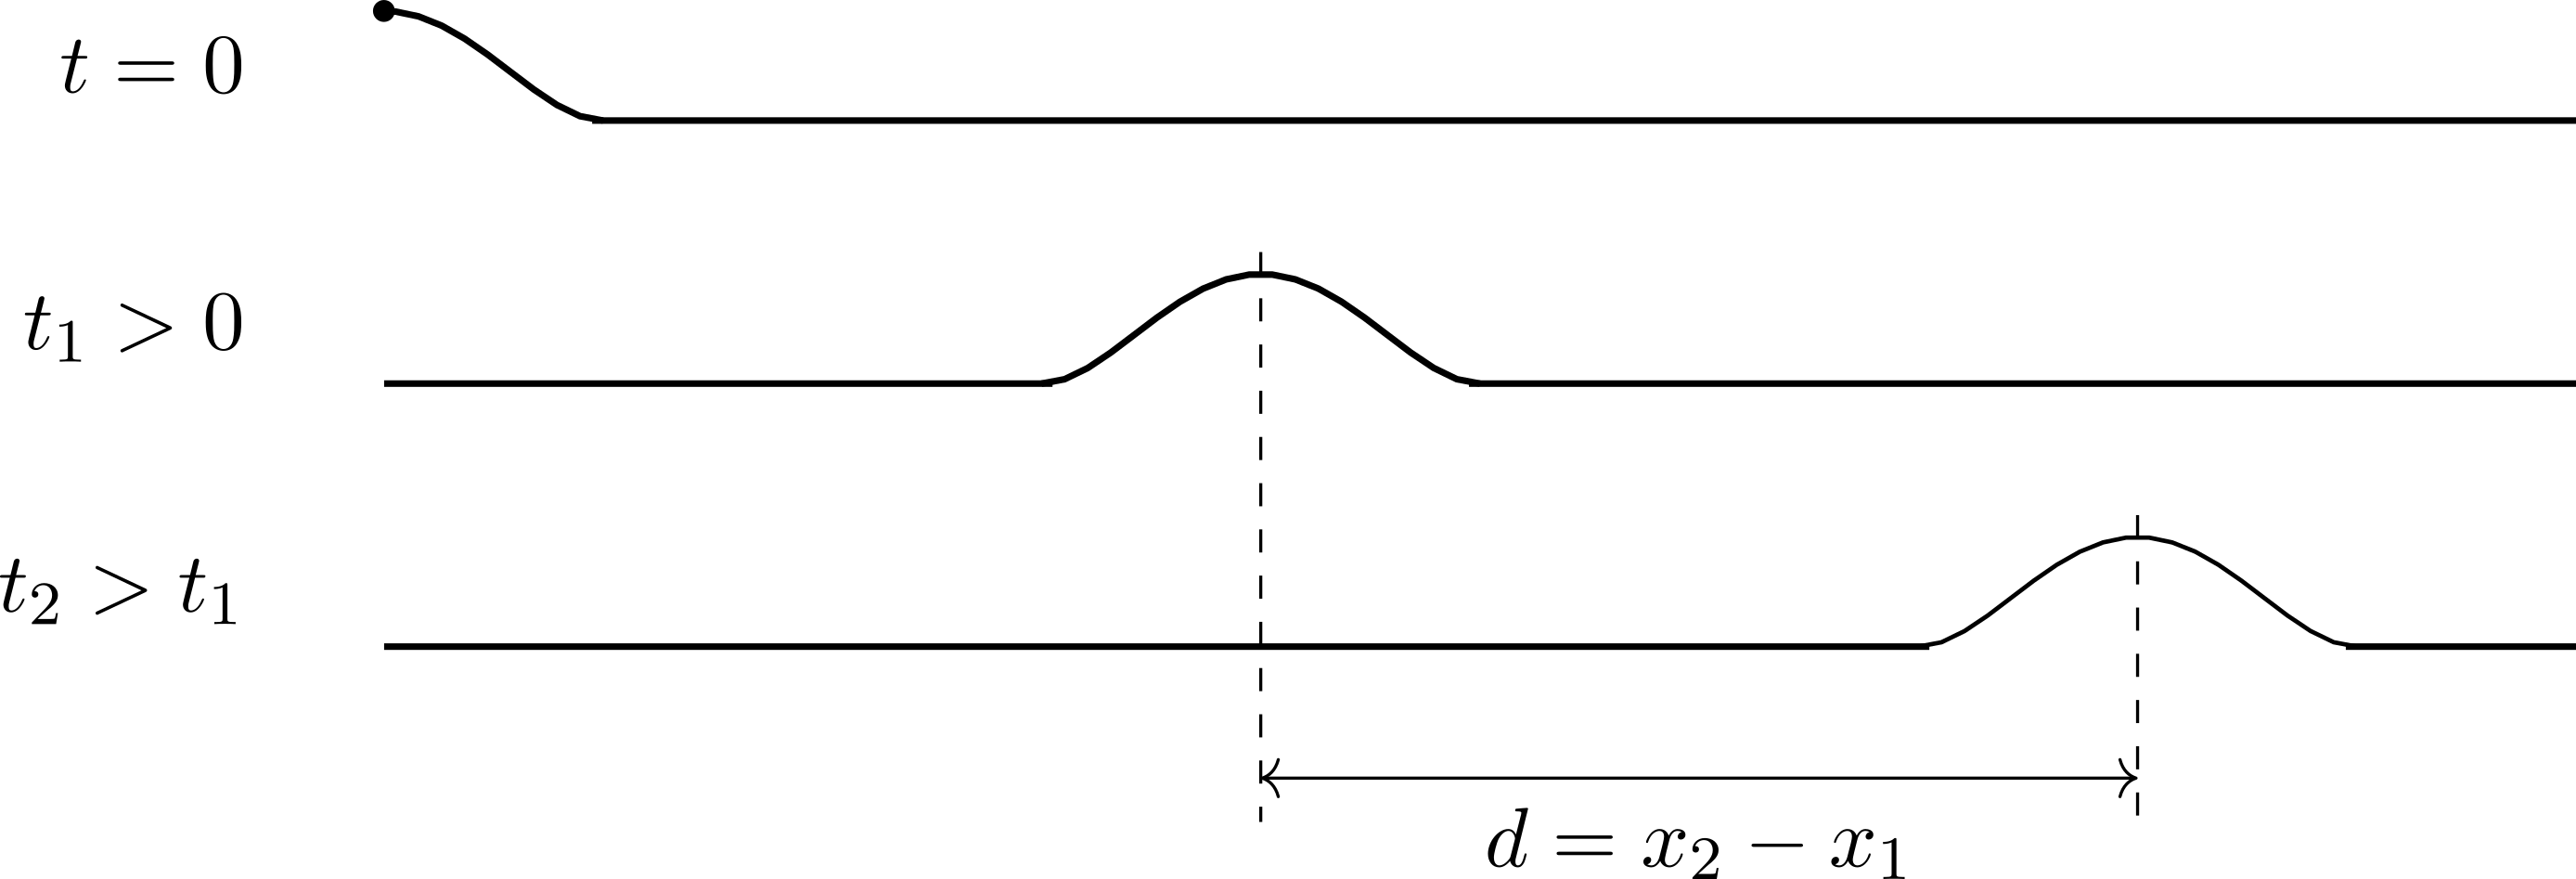
\includegraphics[width=\linewidth, draft=true]{rep_spa}
		}{
			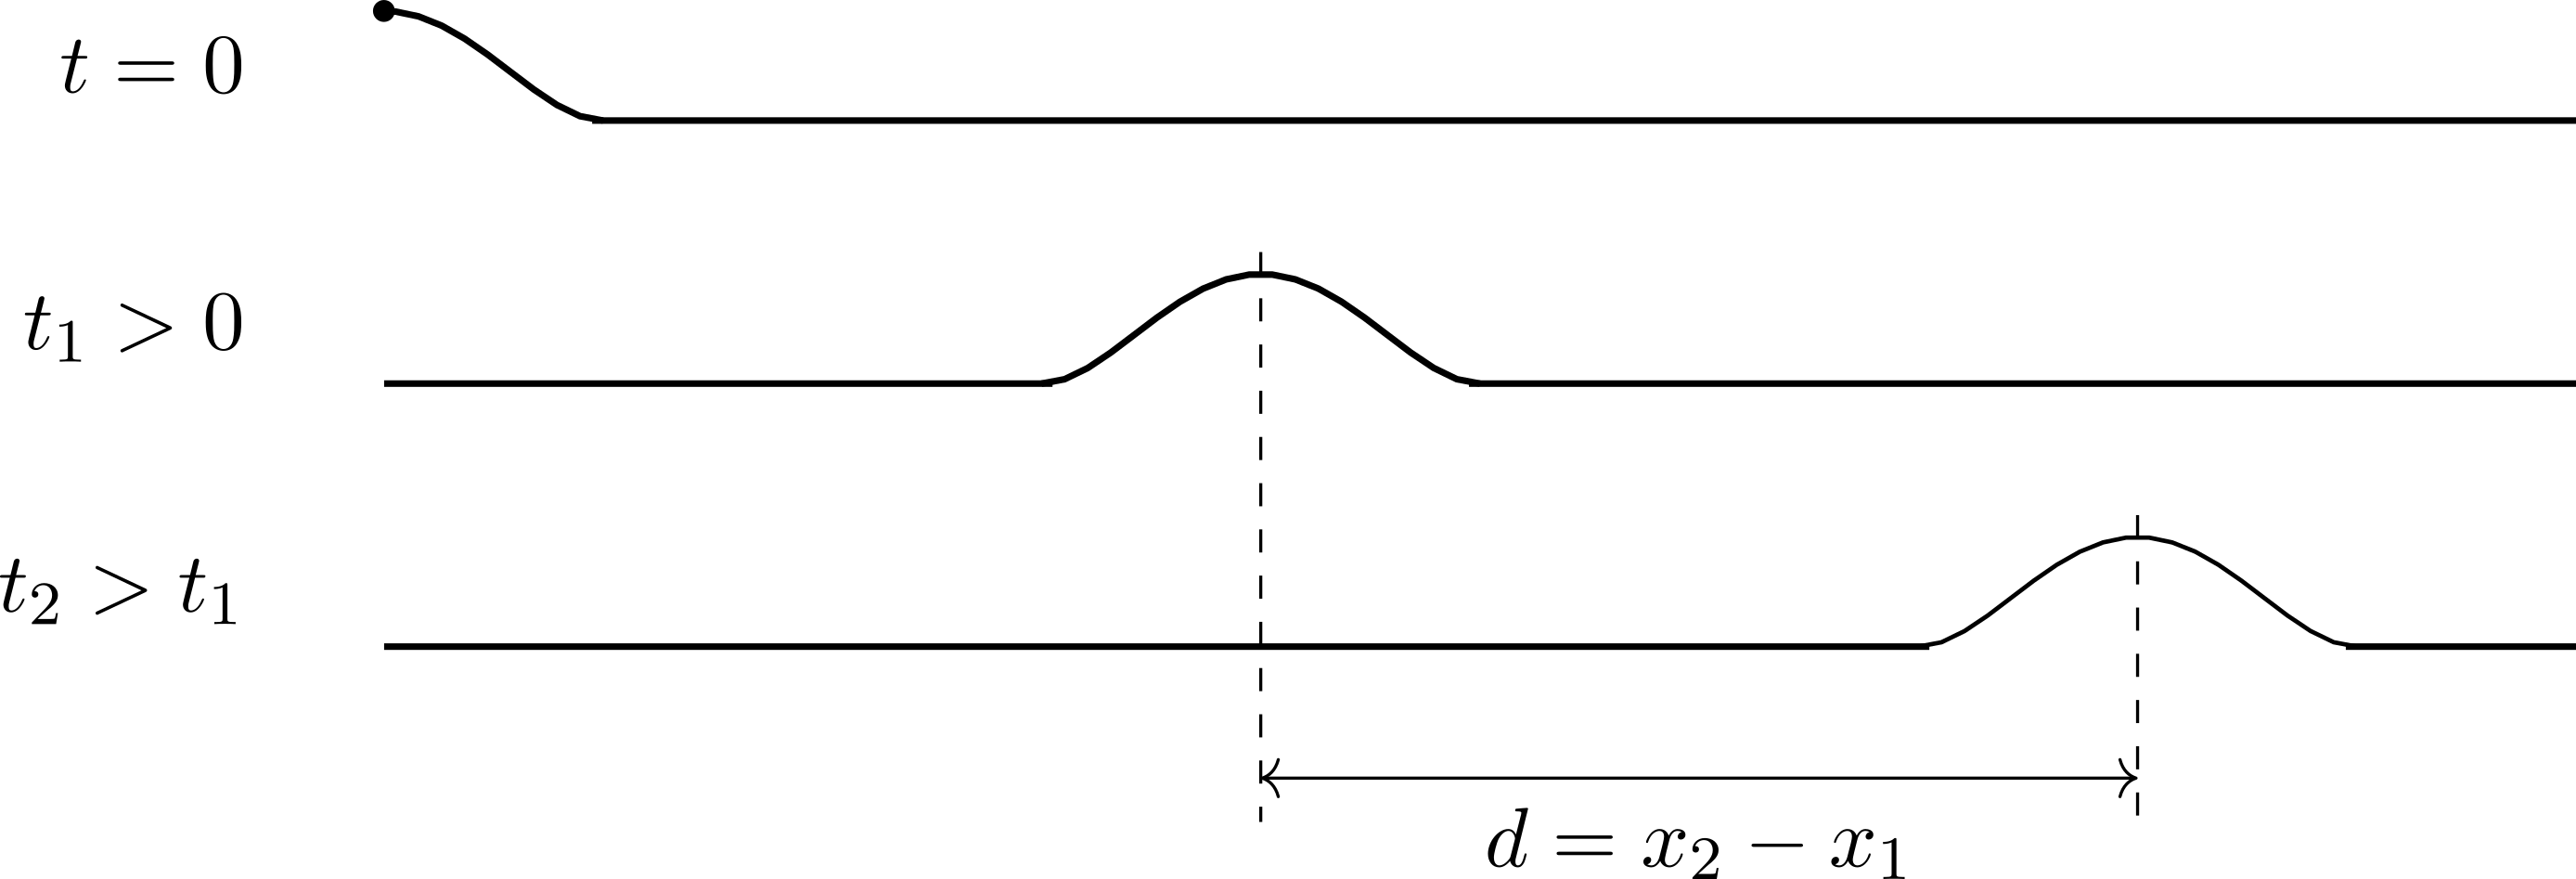
\includegraphics[width=\linewidth]{rep_spa}
		}
		\vspace{-15pt}
		\captionof{figure}{Exemple représentation spatiale}
	\end{center}
\end{tcb}

Lorsqu'une onde se propage, on peut définir une \textbf{vitesse de propagation de la
	perturbation}. Pour la distinguer de la vitesse d'un point matériel, on emploi
plutôt le terme \textbf{célérité}. Par convention, celle-ci est toujours positive.

\begin{tcb}(defi){Définition}
	La célérité $c$ d'une onde est le quotient de la distance $d$ parcourue par la
	perturbation, sur l'intervalle de temps $\Delta t$ que dure ce parcours~:
	\psw{
		\[\boxed{c = \frac{d}{\Delta t}}\]
	}
	\vspace{-15pt}
\end{tcb}

Sur le schéma précédent,
\psw{
	\[
		\boxed{c = \frac{x_2-x_1}{t_2-t_1}}
	\]
}
En première approximation, la célérité ne dépend pas de la perturbation mais
seulement de la nature et des propriétés du \textbf{milieu}.
\begin{table}[h]
	\centering
	\caption{Ordres de grandeur de célérité à connaître}
	\label{tab:ctoknow}
	\begin{tabularx}{.6\linewidth}{lY}
		\toprule
		Signal                   & Célérité
		\\\midrule
		Ondes électromagnétiques & \psw{$\SI{3.0e8}{m.s^{-1}}$}
		\\
		Son dans l'air (\SI{20}{\degreeCelsius},
		\SI{1}{bar})             & \psw{$\approx \SI{340}{m.s^{-1}}$}
		\\
		Son dans les métaux      & \psw{quelques $\si{km.s^{-1}}$}
		\\
		Son dans l'eau           & \psw{$\SI{1.5}{km.s^{-1}}$}
		\\\bottomrule
	\end{tabularx}
\end{table}

\begin{tcb}(appl){Application}
	% Un mascaret est une vague solitaire remontant un fleuve au voisinage de son
	% estuaire, et provoqué par une interaction entre son écoulement et la marée
	% montante.
	On considère ici une vague solitaire qui se déplace à la vitesse $\boxed{c =
			\SI{18}{km.h^{-1}}}$ le long d'un fleuve rectiligne, et on définit un axe
	$(Ox)$ dans la direction du sens de sa propagation.

	À l'instant $t=0$, le profil du niveau de l'eau du fleuve a l'allure
	suivante~:
	\begin{center}
		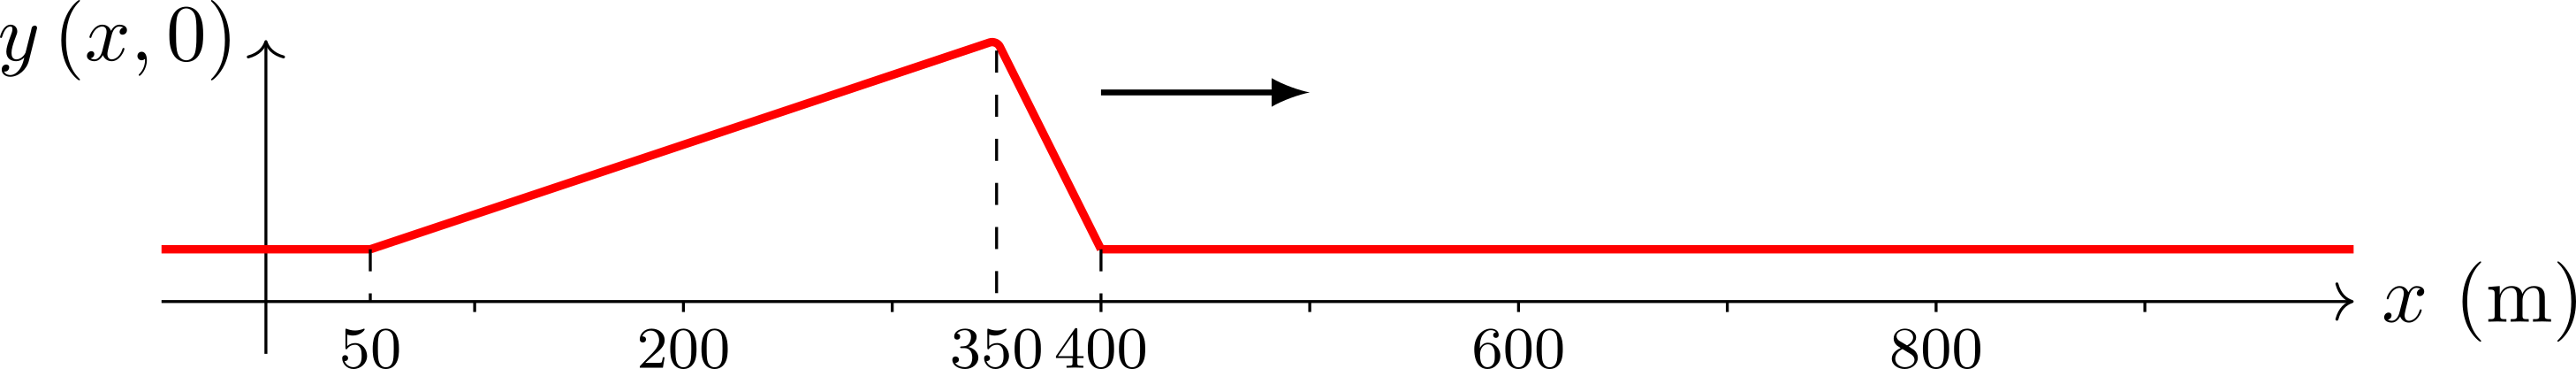
\includegraphics[width=0.8\linewidth]{rep_spa-masc_a}
	\end{center}
	Faire un schéma du profil du fleuve à $\tau = \SI{1}{min}$ en supposant que
	l'onde se propage sans déformation.
	\tcblower
	\psw{
		La queue de la vague est à $x_{q,0} = \SI{50}{m}$. À $\tau =
			\SI{1}{min}$, elle est en $x_{q,1}$. Par définition de la célérité,
		\begin{gather*}
			\frac{x_{q,1}-x_{q,0}}{\tau-0} = c
			\Lra
			x_{q,1} = x_{q,0} + c\tau = \SI{350}{m}
		\end{gather*}
		On procèderait de même pour repérer le haut de la vague et sa tête~: en
		réalité, chaque point du mascaret se déplace de $c\tau = \SI{300}{m}$
		vers la droite.}
	\begin{center}
		\sswitch{
			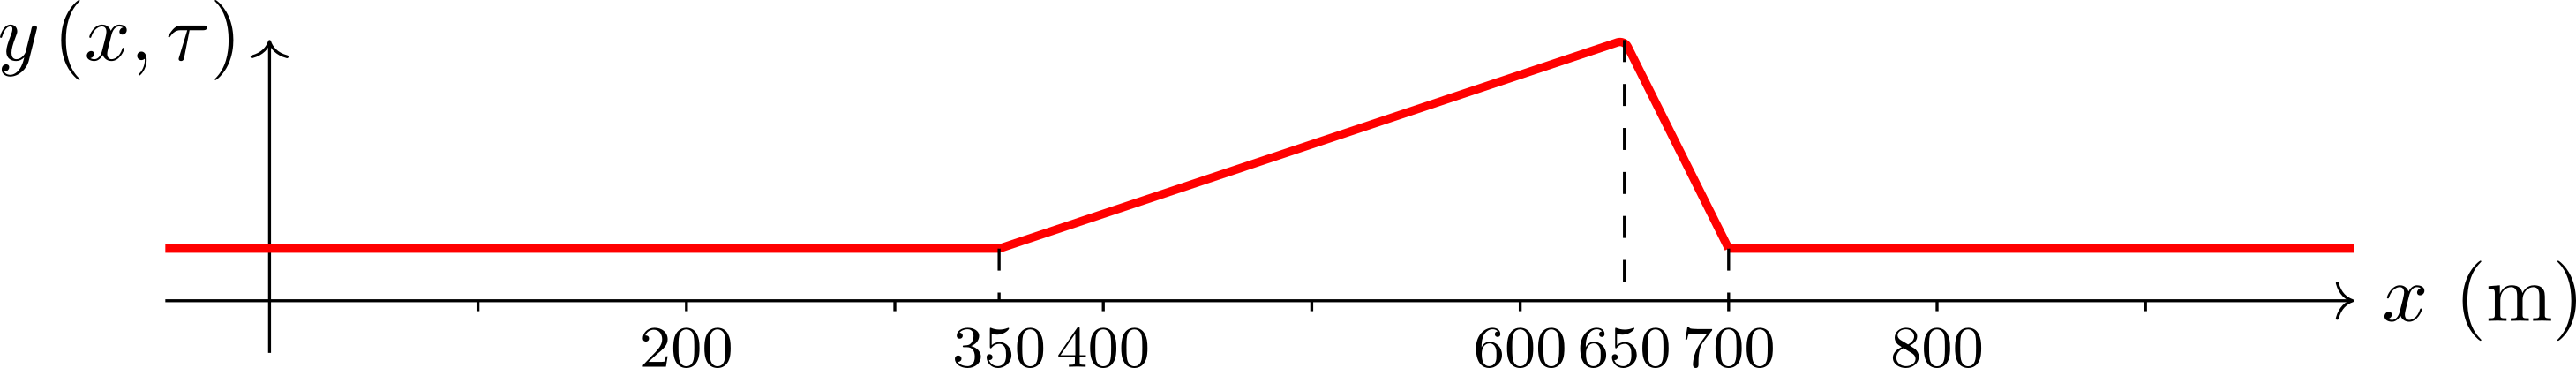
\includegraphics[width=0.8\linewidth, draft=true]{rep_spa-masc_b}
		}{
			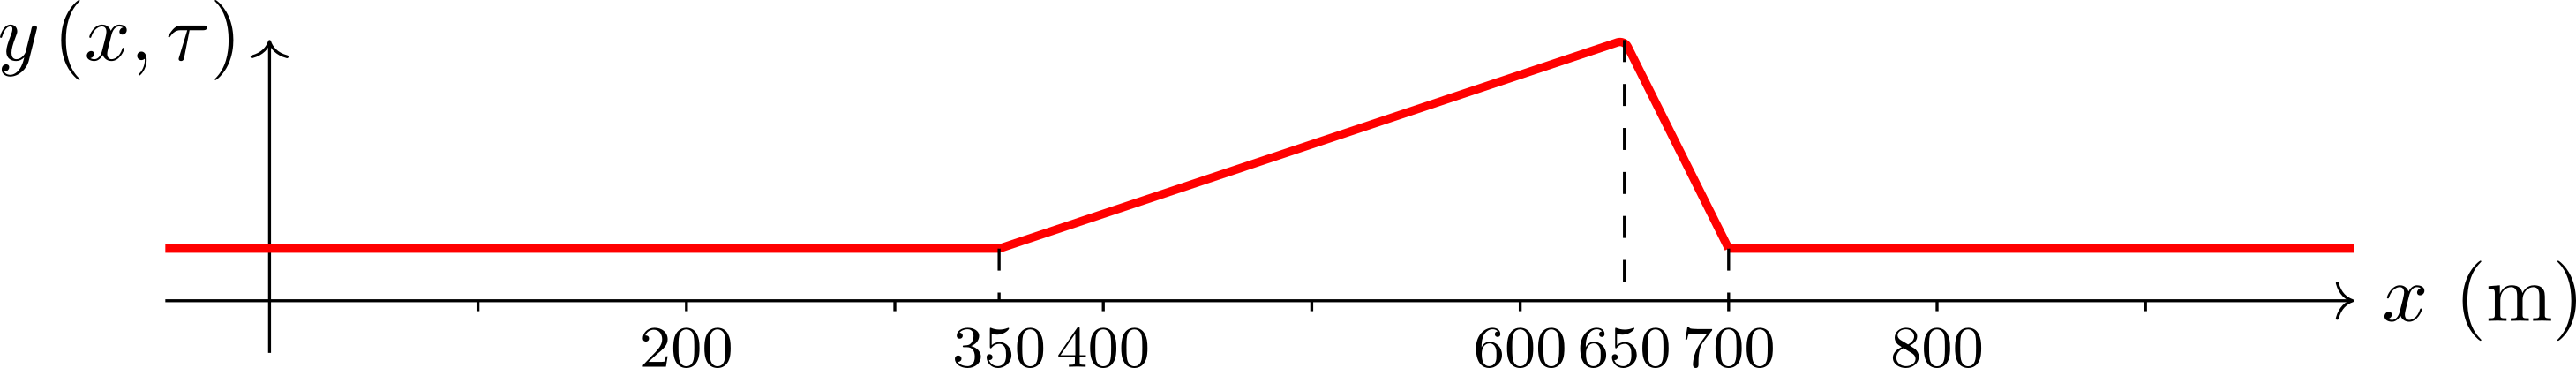
\includegraphics[width=0.8\linewidth]{rep_spa-masc_b}
		}
		\captionof{figure}{Vague solitaire à $\tau = \SI{1}{min}$}
	\end{center}
\end{tcb}

\subsection{Représentation temporelle et retard}

\begin{tcb}(ror){Définition}
	\psw{Dans une représentation \textbf{temporelle}, on regarde à un
		\textbf{endroit fixé} la perturbation \textbf{sur sa durée}. Voir cette
		animation\footnote{\url{https://phyanim.sciences.univ-nantes.fr/Ondes/general/evolution_temporelle.php}}.}
\end{tcb}

On crée à l'instant $t = 0$ une déformation à un endroit M. Cette perturbation se
propage le long d'une corde avec une célérité $c$. Elle parvient en un point
M$_0$, situé à une distance $D$ de M au temps $t_1$ tel que~:
\psw{\[t_1 = \frac{\rm MM'}{c}\]}
\vspace{-15pt}

\begin{tcb}(defi){Définition~: retard}
	\psw{
		La grandeur $\tau$ est le retard du point M' par rapport au point M~:
		\[\tau = \frac{\rm MM'}{c}\]
		avec $c$ la célérité de l'onde.}
\end{tcb}

\begin{tcb}(appl){Application}
	On reprend l'exemple de la vague précédente.
	\begin{enumerate}
		\item À quel instant la vague arrive-t-elle au point d'abscisse $x_1 =
			      \SI{2.2}{km}$~?
		      \smallbreak
		      \psw{
			      À $t=0$, la tête de la vague est à $x_0 = \SI{400}{m}$. Elle
			      arrive en $x_1$ avec un retard~:
			      \[t = \frac{x_1-x_0}{c} = \SI{6}{min}\]
		      }
		      \vspace{-15pt}
		\item Un détecteur fixe, enregistrant la hauteur du fleuve en fonction
		      du temps, est placé à l'abscisse $x_d = \SI{1.6}{km}$. Dessiner
		      l'allure des variations $y(x_d,t)$ en fonction du temps à cette
		      abscisse.
		      \smallbreak
		      \psw{
			      La tête de la vague arrive avec un retard~:
			      \[\tau_{\text{tête}} = \frac{x_d - x_{t,0}}{c} = \SI{4}{min}\]
			      Le haut de la vague arrive avec un retard~:
			      \[\tau_{\text{haut}} = \frac{x_h - x_{h,0}}{c} =
				      \SI{4}{min}\SI{10}{s}\]
			      La queue de la vague arrive avec un retard~:
			      \[\tau_{\text{queue}} = \frac{x_q - x_{q,0}}{c} =
				      \SI{5}{min}\SI{10}{s}\]
		      }
	\end{enumerate}
	\begin{center}
		\sswitch{
			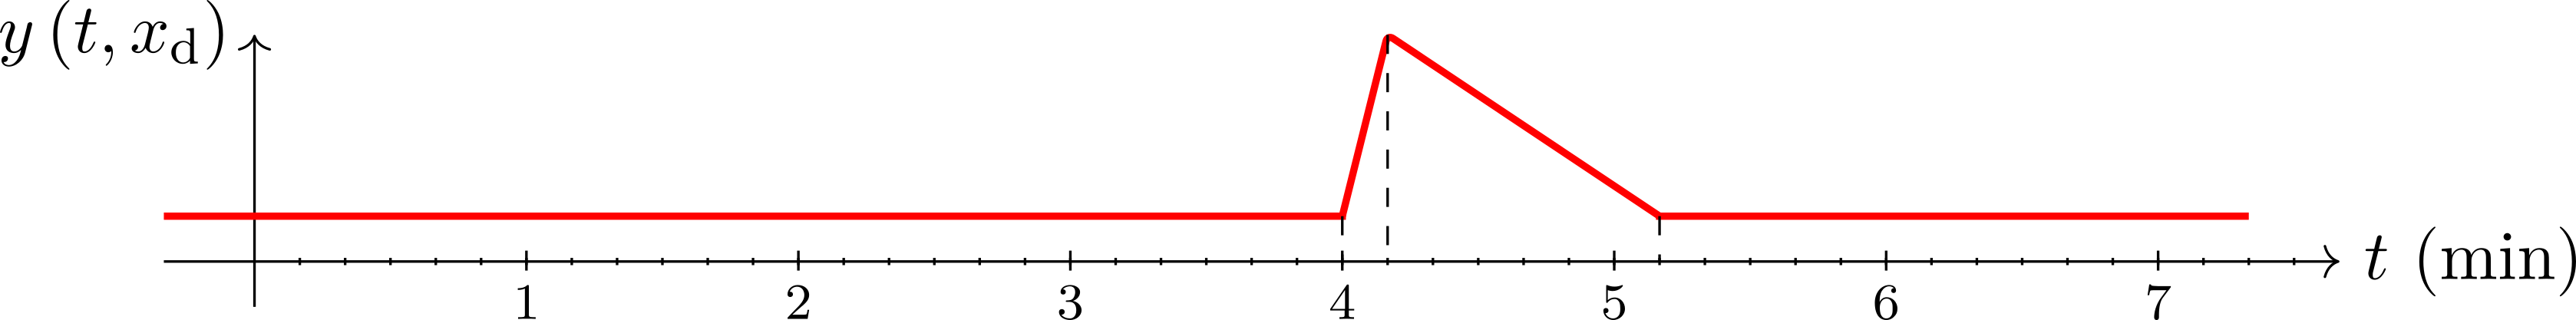
\includegraphics[width=0.8\linewidth, draft=true]{rep_temp_masc}
		}{
			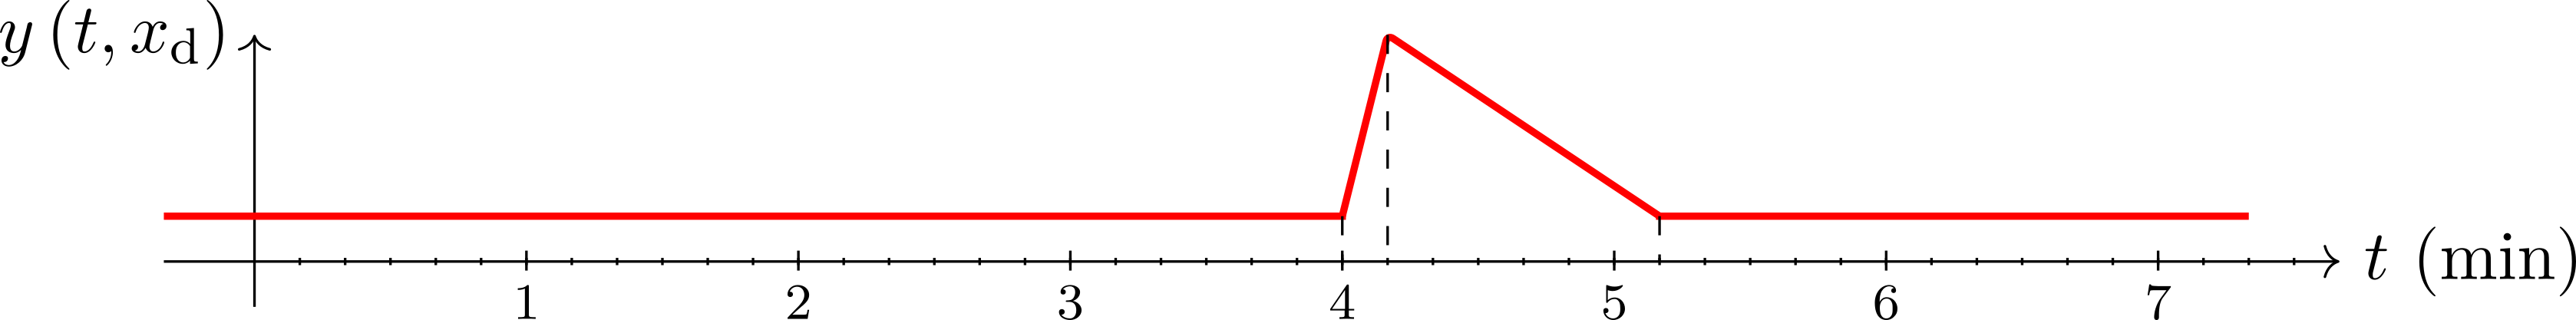
\includegraphics[width=0.8\linewidth]{rep_temp_masc}
		}
		\captionof{figure}{Vague solitaire en représentation temporelle.}
	\end{center}
\end{tcb}

\subsection{Lien entre les représentations}
Nous avons vu deux représentations graphiques différentes, une selon l'espace et
une selon le temps. En réalité, le signal d'une onde est une fonction de
\textbf{deux} variables~:
\[y(x,t)\]
Pour obtenir l'une au l'autre des représentations, on fixe l'une des variables.
Une animation sur les représentations temporelles et spatiales est disponible au
lien suivant~: \url{https://www.geogebra.org/m/RkmRF9M6}

\subsection{Formes mathématiques des représentations}
\subsubsection{À partir de la représentation spatiale}
L'onde observée à $t=0$ se déplace vers la droite. À l'instant $t$, elle est
décalée vers la droite de $\boxed{\psw{\delta = ct}}$~: la valeur de $y(x,t)$
en $x$ et à l'instant $t$ était en $x-ct$ à l'instant $t=0$, soit~:
\psw{
	\[
		y(x,t) = y(x-ct,0)
	\]
}
On note alors $f(x) = y(x,0)$~: c'est la représentation spatiale de l'onde à
$t=0$. On a alors
\psw{
	\[\boxed{
			y(x,t) = f(x-ct)
		}\]
}\vspace{-20pt}
\subsubsection{À partir de la représentation temporelle}

Lorsqu'une onde se propage sans atténuation ni déformation, les valeurs
observées en $x = 0$ au cours du temps sont aussi observées en $x > 0$ mais avec
un retard $\boxed{\psw{\tau = \DS\frac{x}{c}}}$ lié à la propagation.
La valeur de $y(x, t)$ en $x$ à l'instant $t$ était en $x = 0$ plus tôt, à
l'instant $t - x/c$. Ainsi,
\psw{
	\[
		y(x,t) = y\left(0,t-\frac{x}{c}\right)
	\]
}
La fonction $y(0,t)$ est la hauteur de la perturbation en $x=0$ à l'instant
$t$~: c'est la perturbation imposée par la source. On la note alors $g(t) =
	y(0,t)$~: c'est la représentation temporelle de l'onde à $x=0$. On a alors
\psw{
	\[\boxed{
			y(x,t) = g\left(t-\frac{x}{c}\right)
		}\]
}

\begin{tcb}[sidebyside](ror){Conclusion}
	La représentation \textbf{spatiale en $\mathbf{t_0}$} est le graphique de la fonction $x
		\mapsto y(x,t_0)$, soit~:
	\psw{
		\[x\mapsto f(x-ct_0) = g\left(t_0 - \frac{x}{c}\right)\]
	}
	\vspace{-15pt}
	\tcblower
	La représentation \textbf{temporelle en} $\mathbf{x_0}$ est le graphique de la fonction $t
		\mapsto y(x_0,t)$, soit~:
	\psw{
		\[t\mapsto f(x_0-ct) = g\left(t - \frac{x_0}{c}\right)\]
	}
\end{tcb}

\begin{tcb}(impo){Vers la droite ou vers la gauche~?}
	Vous ferez bien attention, à défaut de travailler votre intuition pour
	comprendre que $f (x-ct)$ est une onde se propageant vers la droite, à ne pas
	penser «~signe moins donc vers la gauche~»~! Il faudrait refaire le
	raisonnement, et on arrive à~:
	\smallbreak
	\begin{isd}
		\tcbsubtitle{\fatbox{Vers la gauche}}
		\psw{
			\[
				f (x+ct) = g \left( t + \frac{x}{c} \right)
			\]
		}
		\tcblower
		\tcbsubtitle{\fatbox{Vers la droite}}
		\psw{
			\[
				f (x-ct) = g \left( t - \frac{x}{c} \right)
			\]
		}
	\end{isd}
\end{tcb}

\section{Onde progressive sinuso\"idale}
\subsection{Définition}

\begin{tcb}(defi){Définition~: OPS}
	\psw{
		Une onde progressive est dite \textbf{sinusoïdale} si la source impose une
		\textbf{perturbation sinusoïdale} au milieu.
	}
\end{tcb}

Si on relie un haut-parleur à un GBF délivrant une tension sinusoïdale, on
observe le mouvement périodique dont est animé la membrane de l'air, qui génère
une perturbation périodique de l'air.

% L'exemple du diapason discuté chapitre E7 est également une onde progressive
% sinusoïdale~: lorsque l'on frappe le diapason, celui-ci vibre a une fréquence
% bien déterminée, qui se propage ensuite dans l'air pour parvenir à nos oreilles.

\subsection{Double périodicité spatiale et temporelle}
\subsubsection{Observations sur l'animation \texttt{Geogebra}}
\begin{enumerate}
	\item
	      \psw{
		      Lorsque l'on impose une excitation sinusoïdale, la représentation
		      spatiale est aussi sinusoïdale.
	      }
	\item
	      \psw{
		      À célérité constante, lorsque la fréquence de l'excitation
		      augmente (la période diminue), la période spatiale diminue.
	      }
	\item
	      \psw{
		      À fréquence de l'excitation constante, si on augmente la célérité,
		      la période spatiale diminue.
	      }
\end{enumerate}

\subsubsection{Périodicité temporelle}
Si la perturbation créée en S est sinusoïdale avec une période $T$, alors l'onde
en M l'est également (il n'y a qu'un retard entre les deux dû à la propagation).

\subsubsection{Périodicité spatiale}

Au moment de l'émission du deuxième maximum, le premier maximum a déjà parcouru
une distance $cT$. L'écart entre deux maximum successifs est la période spatiale
soit~:
\[\lambda = cT\]

\begin{tcb}(ror){Bilan}
	\psw{
		Une onde progressive sinusoïdale présente à la fois une périodicité
		spatiale et une périodicité temporelle. La période temporelle $T$ et la
		période spatiale, nommée longueur d'onde et notée $\lambda$, sont
		reliées par la relation
		\[\boxed{\lambda = cT = \frac{c}{f}}\]
		avec $c$ la célérité de l'onde.
	}
\end{tcb}

Cette relation ne vous est sûrement pas inconnue~: c'est de cette manière qu'on
définit à la fois la fréquence (temporelle) et la période (spatiale) d'une onde
électromagnétique, donnant les domaines connus rappelés ci-dessous~:

\begin{center}
	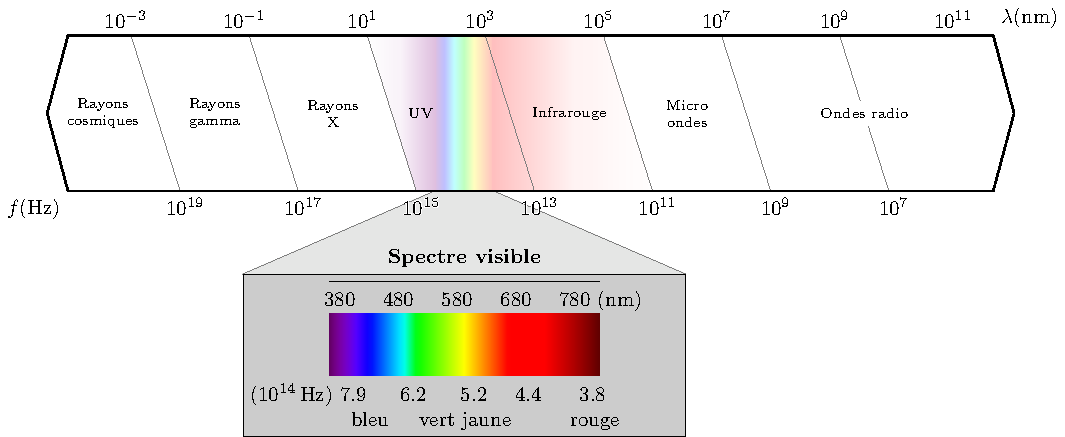
\includegraphics[width=\linewidth]{full_spectre}
\end{center}

\subsection{Expression mathématique de l'onde progressive sinusoïdale}

On s'intéresse à un mouvement vers la droite. Par définition, la perturbation
$g(t)$ imposée en $x=0$ est un signal sinusoïdal~:
\[\psw{g(t) = A\cos(\wt+\f)}\]
\begin{align*}
	\beforetext{Ainsi,}
	\psw{s(x,t)}~ &
	\psw{= A\cos\left(\w\left(t - \frac{x}{c}\right) +\f\right)}
	\\\Lra
	\psw{s(x,t)}~ &
	\psw{= A\cos\left(\wt - \frac{\w}{c}x +\f\right)}
	\\\Lra
	\psw{s(x,t)}~ &
	\psw{= A\cos\left(\wt - \frac{2\pi}{cT}x +\f\right)}
\end{align*}

\begin{tcb}(defi){Définition}
	Comme pour la fréquence et la pulsation, on relie la longueur d'onde à une
	autre grandeur permettant une expression simple dans une fonction
	sinusoïdale~: le \textbf{vecteur d'onde} $k$, tel que
	\[\psw{\boxed{k = \frac{2\pi}{\lambda} = \frac{\w}{c}}
			\qavec
			k\quad\text{en}\quad\boxed{\si{rad.m^{-1}}}}\]
\end{tcb}
\begin{tcb}(prop){Propriété}
	L'expression générale d'une onde progressive sinusoïdale se propageant
	\textit{vers la droite} sans déformation ni atténuation est~:
	\psw{
		\begin{gather*}
			\boxed{s(x,t) = A\cos \left(\wt - kx + \f \right)}\\
			\Lra
			s(x,t) = A\cos \left( \frac{2\pi}{T}t - \frac{2\pi}{\lambda}x + \f
			\right)
		\end{gather*}
	}
	\vspace{-10pt}
\end{tcb}

\begin{tcb}(exem)<lft>'l'{Application}
	On peut vérifier la double périodicité de l'onde ($T$ et $\lambda$). Vérifer
	par exemple la périodicité spatiale.~: soit un signal $s (x,t)$
	double-périodique. Montrer que $s (x+\lambda,t) = s (x,t)$.
	\tcblower
	\psw{
		\begin{align*}
			s(x+\lambda,t) & = A\cos(\wt - k(x+\lambda) + \f)                      \\
			\Lra
			s(x+\lambda,t) & = A\cos\left(\wt - kx - \frac{2\pi}{\lambda}\lambda +
			\f\right)                                                              \\
			\Lra
			s(x+\lambda,t) & = A\cos(\wt - kx -2\pi +\f)                           \\
			\Lra
			s(x+\lambda,t) & = A\cos(\wt - kx +\f)                                 \\
			\Lra
			\Aboxed{
			s(x+\lambda,t) & = s(x,t)
			}
		\end{align*}
	}\vspace{-20pt}
\end{tcb}

\subsection{Vitesse de phase}

Soit une onde progressive sinusoïdale. La \textbf{phase} de l'onde est, par
définition, le terme à l'intérieur de la fonction~: $\wt-kx+\f$. Cette phase
varie spatialement \textit{et} temporellement, de manières corrélées. Si on
trouve une phase mesurée en $x_1$ à l'instant $t_1$, le signal aura la même
phase en $x_2$ à un instant $t_2$ donnés par la \textbf{vitesse de phase}, notée
$v_\f$, telle que~:
\psw{\[\boxed{v_\f = \frac{x_2-x_1}{t_2-t_1}}\]}
\vspace{-10pt}
\begin{tcb}[sidebyside](demo){Démonstration}
	\psw{
		\begin{gather*}
			\wt_2-kx_2+\f = \wt_1-kx_1+\f\\
			\Lra
			\w(t_2-t_1) = k(x_2-x_1)\\
			\Lra
			\boxed{v_\f = \frac{x_2-x_1}{t_2-t_1} = \frac{\w}{k}}
		\end{gather*}
	}
	\tcblower
	\centering
	\tcbsubtitle{\fatbox{Unité}}
	\psw{
		Naturellement, la vitesse de phase s'exprime en \fbox{$\si{m.s^{-1}}$}.
	}
	\vspace{-10pt}
\end{tcb}

\section{Milieux dispersifs}

\begin{tcb}(defi){Définition}
	Un milieu est dit \textbf{dispersif} si
	\psw{la célérité $c$ dépend de la fréquence ou de la longueur d'onde.}
	\bigbreak
	Si c'est le cas, les différentes composantes spectrales d'un signal ne vont
	pas à la même vitesse, et donc le signal peut se déformer lors de la
	propagation.
\end{tcb}
\begin{tcb}[breakable](exem){Exemples}
	\tcbsubtitle{\fatbox{Propagation non-dispersive}}
	\begin{itemize}
		\item
		      \psw{
			      Propagation des ondes acoustiques dans un fluide. La célérité
			      est~:
			      \[c = \frac{1}{\sqrt{\rho_0\chi_0}}\]
			      avec $\rho_0$ la masse volumique du fluide au repos et $\chi_0$ sa
			      compressibilité.
		      }
		\item
		      \psw{
			      Propagation des ondes électromagnétiques dans le vide~:
			      \[c = \SI{299792458}{m.s^{-1}}\]
			      C'est une des constantes fondamentales de la physique.
		      }
	\end{itemize}
	\tcblower
	\tcbsubtitle{\fatbox{Propagation dispersive}}

	\begin{itemize}
		\item
		      \psw{
			      Propagation des ondes à la surface de l'eau. On a
			      \[\w^2 = gk
				      \qsoit
				      v_\f = \sqrt{\frac{g}{k}}
			      \]
			      Ainsi, la vitesse de phase dépend de $k$, et donc de la longueur
			      d'onde.
		      }
		\item
		      \psw{
			      Propagation des ondes électromagnétiques dans le verre~:
			      \[v_\f = \frac{c}{n(\lambda)}\]
			      avec $n(\lambda) = A + \frac{B}{\lambda^2}$. C'est la dispersion qui
			      cause la décomposition spectrale de la lumière par un prisme.
		      }
	\end{itemize}
	\vspace{-10pt}
\end{tcb}

\sidecaptionvpos{figure}{c}
\begin{SCfigure}[1][h!]
	\centering
	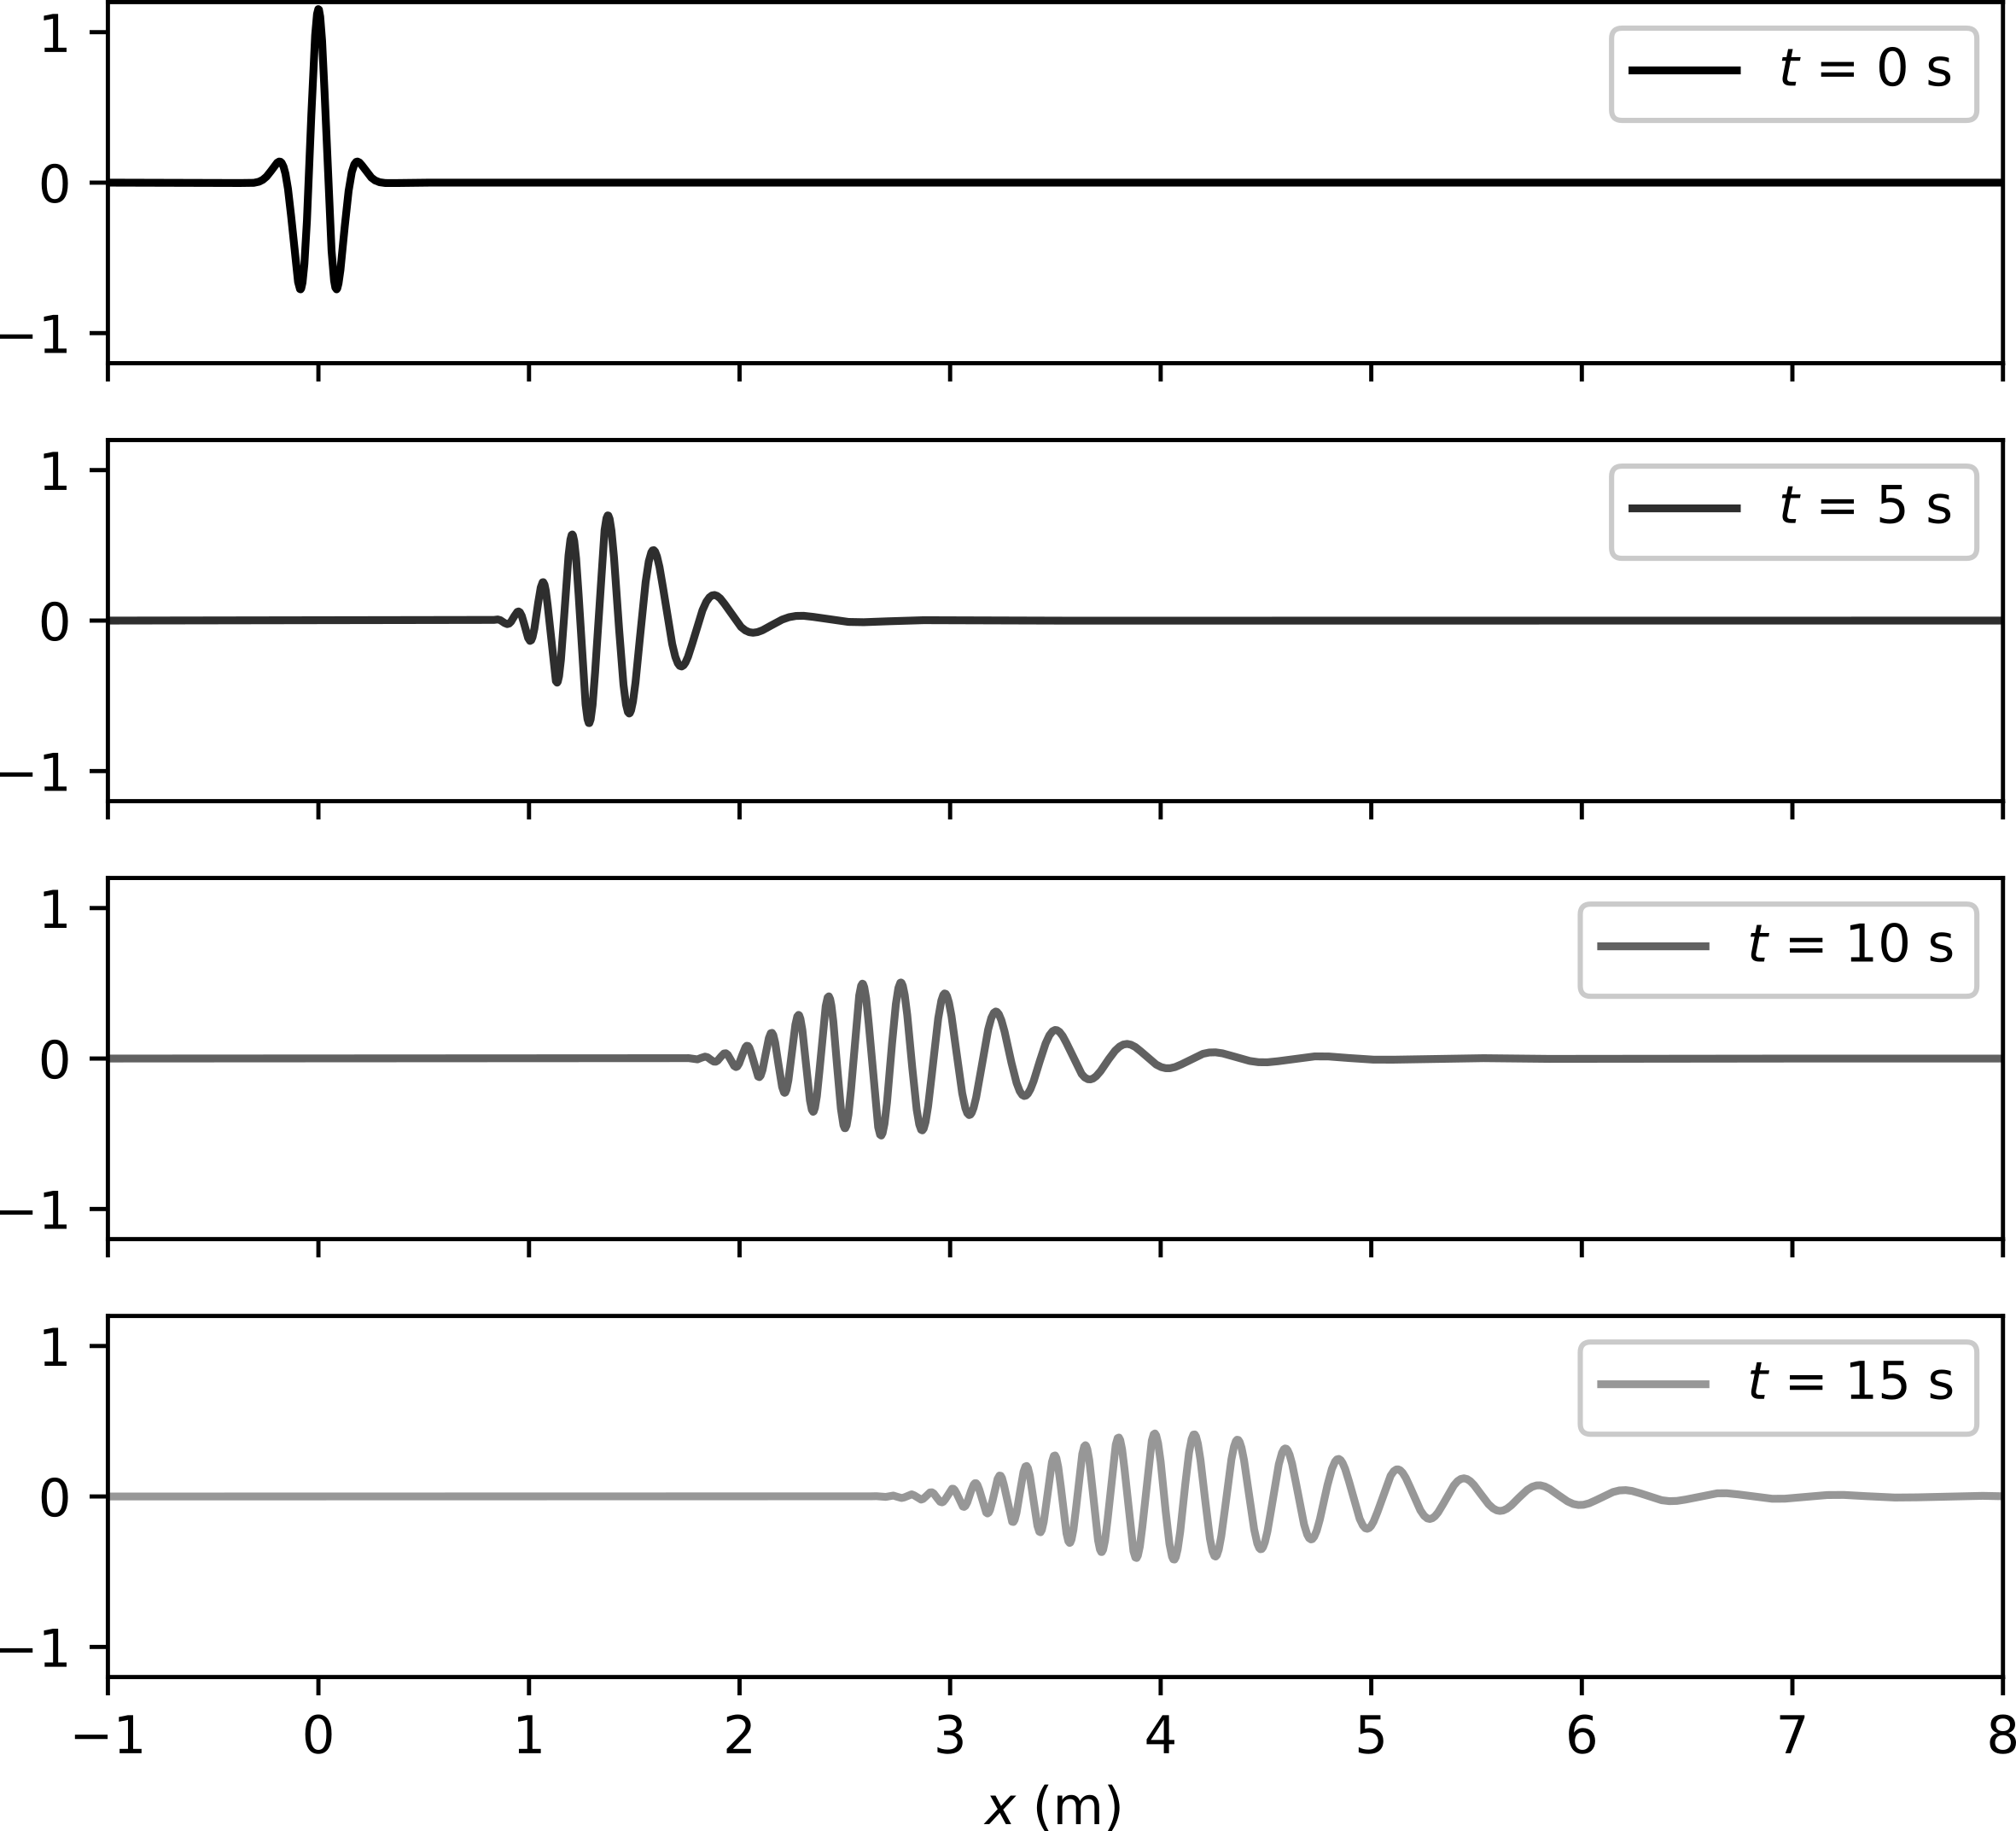
\includegraphics[width=.45\linewidth]{dispersion}
	%\captionsetup{justification=centering}
	\caption[Dispersion d'une onde à la surface de l'eau]{Propagation dispersive
		d'une onde à la surface de l'eau. On observe nettement que les
		composantes sinusoïdales de hautes fréquences se propagent avec une
		moins grande vitesse que les composantes de basses fréquences. En
		ordonnée, l'unité de la hauteur d'eau est arbitraire.}
	\label{fig:disp_eau}
\end{SCfigure}

\end{document}
